%============================================================================================
% DtN operators
%============================================================================================
\documentclass[fleqn]{article}

\usepackage{amssymb}
\usepackage{amsmath}
\usepackage{graphicx}
\usepackage{geometry}
\usepackage{xcolor}
\usepackage{tikz}

\geometry{
  left=20mm, right=20mm, top=20mm, bottom=20mm
}

\begin{document}

\section{Merging DtN operators}

\subsection{Setting}

\begin{figure}[!h]
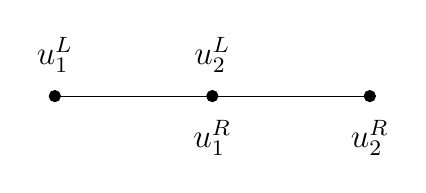
\begin{tikzpicture}

\coordinate (P1) at (0, 0);
\coordinate (P2) at (2, 0);
\coordinate (P3) at (4, 0);

\draw (P1) -- (P2) -- (P3);

\filldraw (P1) circle (2pt);
\filldraw (P2) circle (2pt);
\filldraw (P3) circle (2pt);

\node[yshift=+15pt] at (P1) {\large $u_1^L$};
\node[yshift=+15pt] at (P2) {\large $u_2^L$};
\node[yshift=-15pt] at (P2) {\large $u_1^R$};
\node[yshift=-15pt] at (P3) {\large $u_2^R$};

\end{tikzpicture}
\end{figure}

Left DtN operator:
\begin{subequations}
\begin{align}
N_1^L &= a_{11}^L u_1^L + a_{12}^L u_2^L + b_1^L \\
N_2^L &= a_{21}^L u_1^L + a_{22}^L u_2^L + b_2^L
\end{align}
\end{subequations}

Right DtN operator:
\begin{subequations}
\begin{align}
N_1^R &= a_{11}^R u_1^R + a_{12}^R u_2^R + b_1^R \\
N_2^R &= a_{21}^R u_1^R + a_{22}^R u_2^R + b_2^R
\end{align}
\end{subequations}

\subsection{Bridge solution}

The bridge value:
\begin{equation}
u := u_2^L = u_1^R 
\end{equation}
The bridge solution:
\begin{equation}
u = q_1 u_1^L + q_2 u_2^R + r_{12}
\end{equation}
where
\begin{subequations}
\begin{align}
q_1 &= -\,q_{12}\,a_{21}^L \\
q_2 &= +\,q_{12}\,a_{12}^R
\end{align}
\end{subequations}
and
\begin{equation}
r_{12} = q_{12} \left( b_1^R - b_2^L \right)
\end{equation}
with
\begin{equation}
q_{12} = \left(a_{22}^L - a_{11}^R\right)^{-1}
\end{equation}

\subsection{New DtN operator}

The new operator:
\begin{subequations}
\begin{align}
N_1^L &= a_{11} u_1^L + a_{12} u_2^R + b_1 \\
N_2^R &= a_{21} u_1^L + a_{22} u_2^R + b_2
\end{align}
\end{subequations}
where
\begin{subequations}
\begin{align}
a_{11} &= a_{12}^L q_1 + a_{11}^L \\
a_{12} &= a_{12}^L q_2 \\
a_{22} &= a_{21}^R q_2 + a_{22}^R \\
a_{21} &= a_{21}^R q_1
\end{align}
\end{subequations}
and
\begin{equation}
b_1 = a_{12}^L r_{12} + b_1^L
\end{equation}
\begin{equation}
b_2 = a_{21}^R r_{12} + b_2^R
\end{equation}

\end{document}
